\part{Des données à valoriser}

\clearpage
\thispagestyle{empty}
\cleardoublepage

\chapter{Données graphiques, données statistiques}

\section{Le lien entre le texte et les images du texte}

Dans chaque élément \texttt{<facsimile>}, une balise \texttt{<surface>} définit le bloc de segmentation supérieur (la page). L'élément suivant, \texttt{<graphic>}, indique dans son attribut \texttt{@url} la localisation de l'image de la page segmentée. L'ensemble des images étant stocké dans l'espace alloué au programme \timeus{} au sein du service \sharedocs{} de la TGIR Huma-Num, la localisation consiste en un chemin relatif (\fig{} \ref{fig:facsimile} p. \pageref{fig:facsimile}).

Or ces images sont déjà hébergées par \ia. Elles ont été téléchargées sur le \sharedocs{} dans le but de permettre leur segmentation par \textit{FineReader} et \transkribus{} puis leur \ocr{} par \lse. Leur conservation après l'obtention des fichiers XML n'est plus aussi pertinent que celle des prises de vues effectuées dans des dépôts d'archives, qui n'existent sous aucune autre forme. Rappelons également qu'\ia{} se donne pour objectif d’être un centre stable et durable d’archives digitales ; il est donc peu probable que les images des \odm{} disparaissent de ses serveurs. Il nous a donc été demandé de substituer le chemin local par l'adresse de l'image sur \ia{} (\ann{} \ref{ann:feuille_route}, \issue{} 2) ; cette mission a donné lieu à la publication d'un billet sur le carnet de recherche du programme \timeus\footcite{genero}.

Nous avons apporté deux solutions : l'une employait les URLs basiques des images, l'autre mobilisait les manifestes \iiif{} des volumes. Toutes deux ont donné lieu à des scripts Python dont les fonctionnements sont similaires.

Les URLs se trouvaient dans des fichiers JSON renseignés dans le code source des pages d'\ia. Un fichier JSON contient des informations représentées de manière structurée ; il s'agissait ici de métadonnées concernant le volume numérisé. Parmi celles-ci, une sous-section intitulée \texttt{data} contenait des métadonnées (longueur, largeur, etc.) et l'URI de chaque image. Ces images étaient au format JPEG et correspondaient à celles téléchargées sur le \sharedocs.

Nous n'avons exploré la piste du \iiif{} que dans un second temps, à la suite de plusieurs incitations. L'\textit{International Image Interoperability Framework} permet d'afficher une image avec ses métadonnées dans le contexte d'une application web directement depuis le serveur où elle est conservée (ici, \ia). Les URLs de cette deuxième solution se trouvent dans les \og manifestes \iiif{} \fg{} des volumes : il s'agit des documents JSON contenant leurs métadonnées et référençant les points d'accès aux images (\cad{} leurs URIs dans le protocole \iiif).

Si ces images possèdent le même format que celles de la première solution, leur qualité est bien supérieure et permet d'effectuer des agrandissements d'une très grande profondeur. Du reste, le \iiif{} permet également de naviguer dans un volume en passant de page en page. Cette seconde solution est donc plus intéressante pour le projet \timeus{} dans la mesure où elle lui permet d'accéder d'une manière relativement simple à un document contenant un ensemble de données et de métadonnées qui pourront être valorisés au moment d'une édition en ligne.

Le script dont il est ici question, s'il se limite à insérer les URIs des images dans le code XML, commence par effectuer une requête pour lire le contenu des manifestes \iiif{} des \odm{}. Pour cela, il lit un CSV où nous avons enregistré les identifiants donnés par \ia{} aux numérisations, et les utilise pour compléter l'adresse des manifestes (\texttt{https://iiif.archivelab.org/iiif/<itemid>/manifest.json}). Ces lignes de code peuvent être réutilisées, probablement sous la forme d'une fonction, pour obtenir tout type de métadonnées issues des manifestes. En plus de rationaliser le stockage sur le \sharedocs{}, ce script prépare donc l'étape de la publication en ligne.

\section{Les données graphiques dans le flux textuel}

Un des principaux apport du \iiif{} pourrait être le traitement des objets graphiques qui, nous l'avons vu, sont nombreux dans les pages des \odm{} (\fig{} \ref{fig:ex_figures} p. \pageref{fig:ex_figures}). En particulier, les objets de type photographie, figure ou carte pourrait bénéficier des fonctionnalités d'agrandissement et permettre à l'utilisateur de pleinement les prendre en considération.

Pour rendre cela possible, il faudrait disposer d'une évaluation du taux de détection des figures. Les tableaux sont celles qui ont posé le plus de problème au script, nous y reviendrons. Parmi les autres, plusieurs n'ont été que partiellement détectées. La carte de la page 439 de la monographie 90\footcite{mono090a} est ainsi parfaitement détectée et transposée dans un élément \texttt{<figure>} (\fig{} \ref{fig:odmfig90439}). À l'inverse, le plan d'une \og habitation cambodgienne à Pnom-Penh \fg{} est détecté en double --- peut-être en raison de la superposition d'une vue de face de l'habitation et de son plan --- et le titre de la figure est transcrit comme du texte (\fig{} \ref{fig:odmfig90453}). Dans la monographie suivante\footcite{mono090b}, la photographie pleine page \og Cambodgiens et amanites \fg{}, insérée entre les pages 484 et 485, a été retirée du texte et n'est pas présente dans les fichiers sous quelque forme que ce soit.

\begin{figure}
    \centering
    \begin{subfigure}{0.4\textwidth}
     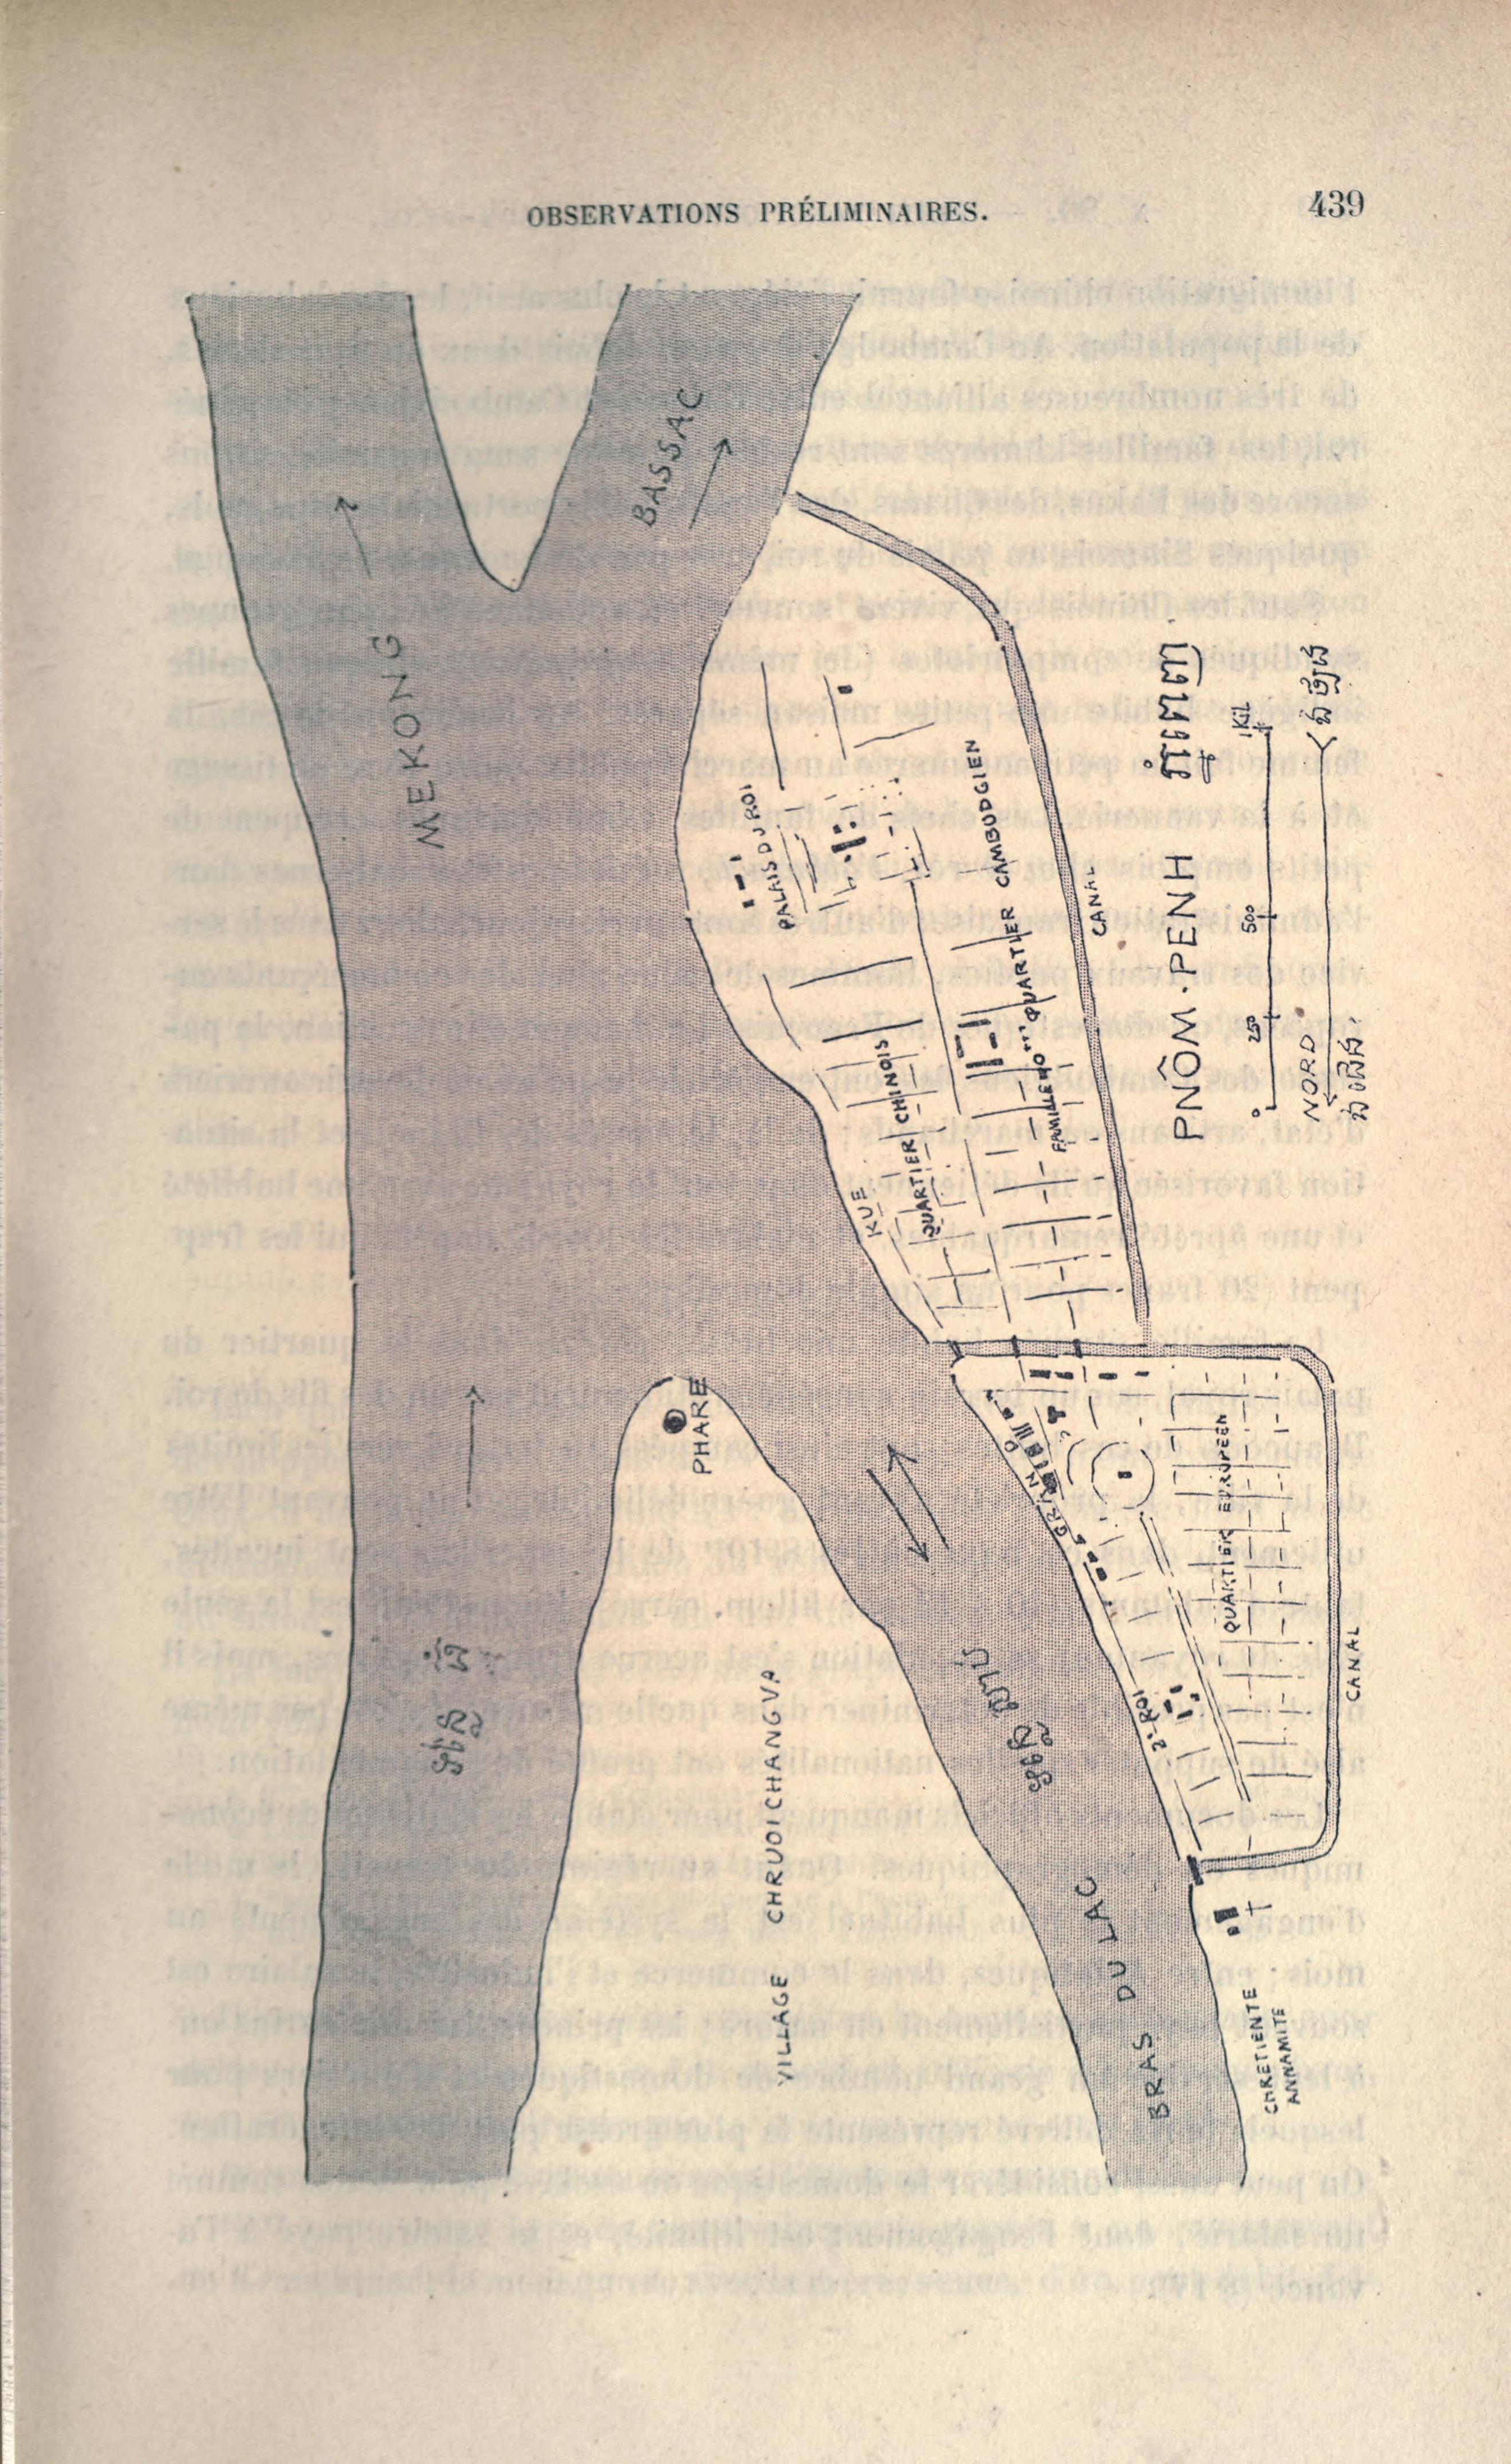
\includegraphics[width=1\linewidth]{img/odm90_439.jpg}
     \caption{Page 439 : détection optimale de la carte.}
     \label{fig:odmfig90439}
    \end{subfigure}
    \hspace{5pt}
    \begin{subfigure}{0.4\textwidth}
     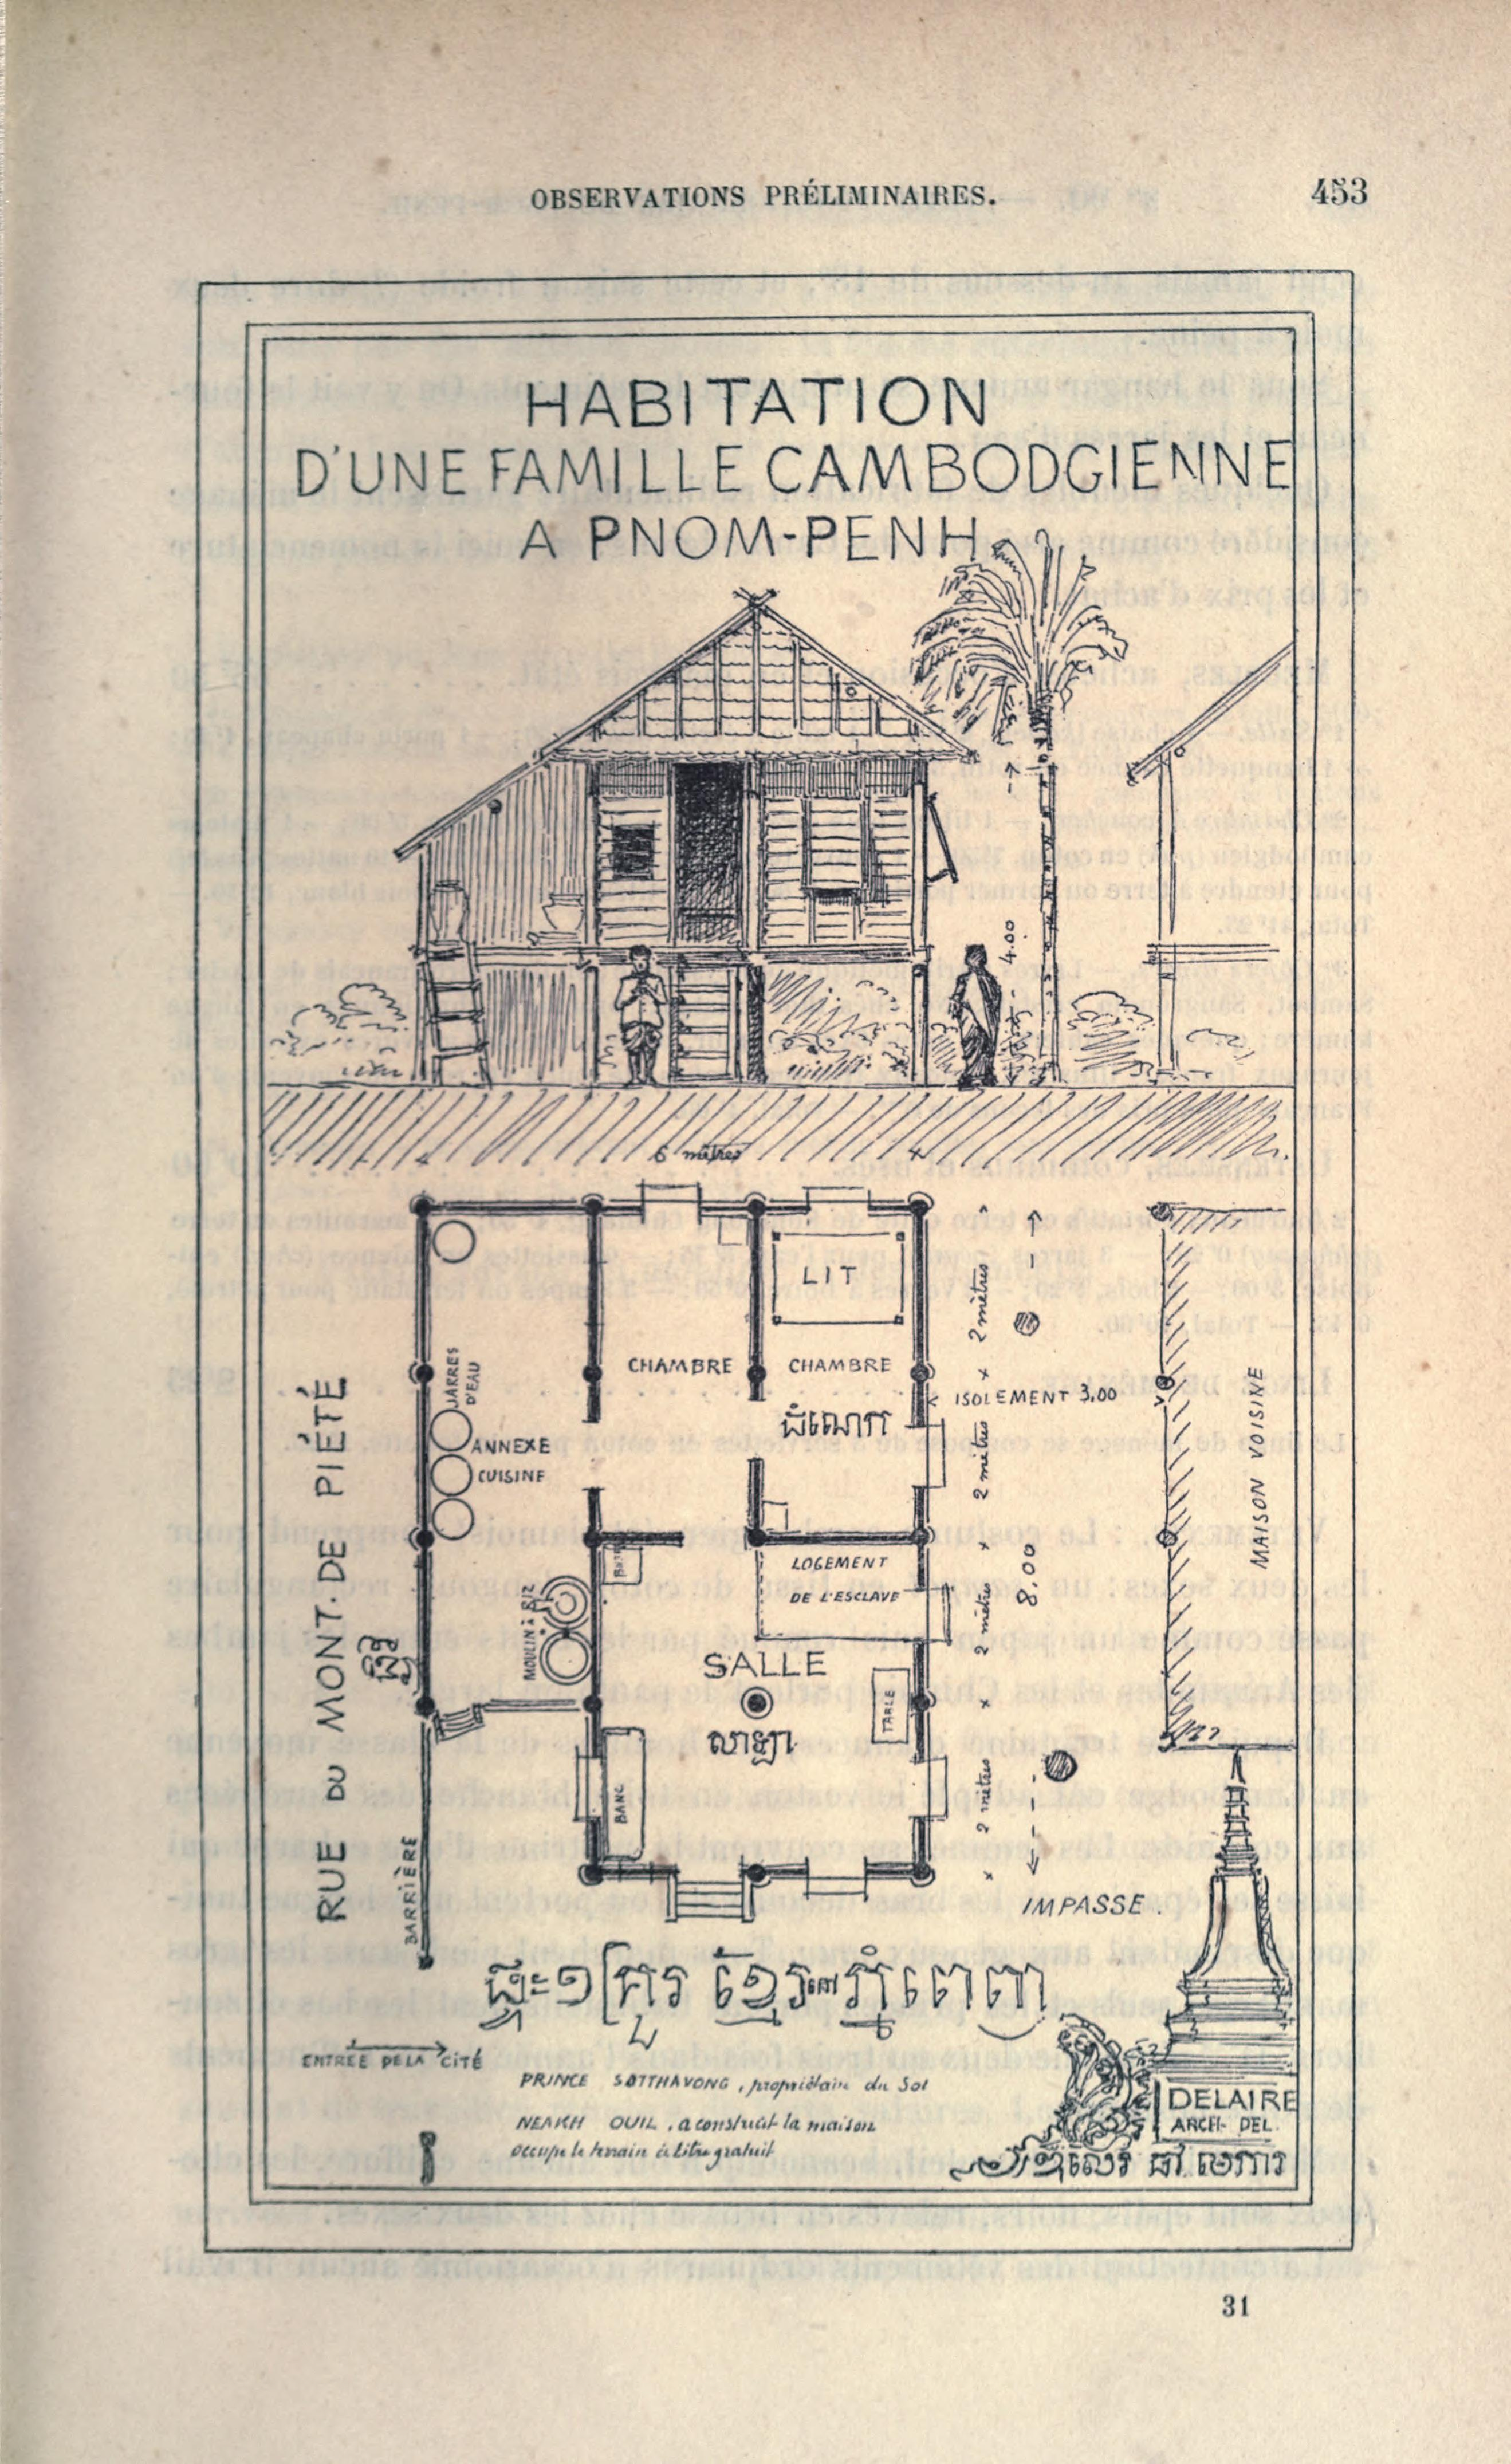
\includegraphics[width=1\linewidth]{img/odm90_453.jpg}
     \caption{Page 453 : détection en double et transcription du titre.}
     \label{fig:odmfig90453}
    \end{subfigure}
    \caption{Figures dans la monographie n° 90.}
    \label{fig:odmfig90}
\end{figure}

Ces erreurs de détection ne peuvent pas être résolues de manière automatique : aucune table des figures n'est présente dans les volumes. Elle eut permis de cibler les pages à contrôler et de ne pas avoir à chercher visuellement les figures. Une intervention manuelle, possiblement longue, s'impose donc.

La présence de ces figures est également un élément à garder à l'esprit au moment de la reconstitution des paragraphes. En effet, certaines sont insérées en plein milieu d'un paragraphe. Pour ne pas perturber la reconstitution, il sera nécessaire d'ajouter une condition spécifiant que les balises \texttt{<p>} commençant pas une minuscule ne constituent pas une unité indépendante, et ce même si elles sont précédées d'une figure. Le problème de cette méthode est qu'elle présuppose que \lse{} a bien fait la différence entre une majuscule et une minuscule, ce dont on ne peut pas 
être totalement certain.

Ajoutons enfin que les figures de type carte, croquis ou photographie ne sont pas importantes du \pov{} de la donnée pure. Elles ne sont pas utiles aux chercheurs qui s'intéressent au vocabulaire du textile ou du monde ouvrier, ni à ceux qui souhaitent recueillir des données chiffrées. Dans le document XML, elles ne sont que des repères dont la nécessité ne se révélera qu'au moment de la transformation des fichiers pour une interface de visualisation.

\section{Les tableaux : une mise en image des données ?}

À l'inverse, les tableaux qui jalonnent le corpus ont une importance considérable en raison des informations statistiques qu'ils contiennent.

Avant de décrire la manière dont \lse{} les a traités, posons nous la question de la manière dont nous pourrions accéder aux données qu'ils contiennent.

\chapter{Données textuelles, données scientifiques}

\chapter{Une valorisation plurielle}

\section{Édition papier, édition numérique}

Un postulat commun veut qu'une édition numérique offre à son utilisateur plus de possibilité qu'une édition papier n'en offre à son lecteur\footnote{\og \textit{Often these descriptions glance at their print predecessors, usually with expressions of how much more these digital editions can contain than ever could be included in print editions, and how much more the reader can do with them} \fg{} : \cite[p. 105-106]{robinson}.}. Le numérique permet en effet de concevoir des plate-formes sur mesure pour la consultation des textes, et les outils des humanités numériques permettent à \og de nombreuses données non interrogeables jusqu’à présent [d'être] l’objet d’enquêtes \fg\footcite[p. 20]{duval}. \og Des structures cachées, des faits de système difficilement décelables à l’œil et à la main \fg{} deviennent ainsi accessibles\footcite{duval}.

Dans le programme \timeus{}, l'édition numérique des \odm{} a éveillé l'intérêt d'au moins trois participants. Le LARHRA de l'université de Lyon 2, dans le strict respect des objectifs du programme, souhaite utiliser les informations économiques fournies par les tableaux de budget et celles d'ordre prosopographique contenues dans le paragraphe \og §2 --- État civil de la famille \fg. L'équipe ALMAnaCH d'Inria a pour sa part la volonté de puiser dans les champs lexicaux des mondes ouvrier et industriel afin d'alimenter des algorithmes de traitement automatique du langage (TAL). Enfin, le Centre de recherches historiques (CRH) veut fournir à la communauté scientifique une édition numérique des \odm{} qui intégrerait des informations matérielles sur la constitution du corpus et le travail de la \sess.

On le voit, les objectifs poursuivis par ces entités sont très divers. Les matériaux qui permettront de les réaliser le sont tout autant : le LARHRA et ALMAnaCH ont besoin de données brutes issues des tableaux statistiques (des chiffres) et du texte (des mots), tandis que le CRH agrège des métadonnées inédites qui proviennent de plusieurs corpus. Le LARHRA a également besoin d'une transcription de qualité pour s'assurer de la viabilité des informations prosopographiques du second paragraphe.

Cette pluralité de directions illustre la tension qui traverse les éditions numériques : elles portent avant tout sur un document et non sur une \oe{}uvre\footnote{\og \textit{Two decades of making digital editions, and recent papers about digital editions, have moved the needle away from the “work” to the “document”, to the point where we might need only think of “documents”} \fg{} : \cite[p. 107]{robinson}}. Cette distinction est issue de la triade document, texte, \oe{}uvre (\textit{document}, \textit{text}, \textit{work}) qui désigne les dimensions matérielle, linguistique et intellectuelle d'un écrit\footnote{\og \textit{Work} désigne le texte de l’auteur, éventuellement le texte correspondant à la volonté de l’auteur, et implique la notion d’authenticité ; \textit{text} dénomme la séquence linguistique attestée dans un document transmettant l’œuvre ; enfin \textit{document} est une manifestation physique d’un text \fg{} : \cite[p. 15-16]{duval}.}. De fait, l'encodage que nous avons décrit dans la partie précédente fait la part belle au document \odm{} de l'Université de Toronto, digitalisé par \ia. \transkribus{} et le script \lse{} mobilisent la TEI pour mener à bien la reproduction fidèle du document grâce à des ensembles \texttt{<facsimile>}\footcite[p. 124]{robinson}. L'\oe{}uvre n'est pas pour autant oubliée. Elle se rencontre dans la structure logique leplaysienne, là encore reproduite fidèlement par le biais des divisions et des titres.

Cette coexistence apparente n'a cependant pas vocation à durer : dans la vision de \timeus, c'est bien l'\oe{}uvre et non le document qui doit prendre le dessus. Il n'est pas question de concevoir un support de consultation qui présenterait des échantillons successifs correspondant au contenu d'une page. Cela reviendrait à reproduire l'interface de visualisation d'\ia, tout en donnant une réalité concrète à l'hypertexte qui est \og en gestation dans les tables, index et diverses aides à la lecture de consultation déjà présentes \fg{} dans les volumes\footcite[p. 19]{duval}.

Le premier essai d'édition des fichiers XML, mené par Alix Chagué, consiste ainsi en un document HTML où l'intégralité du texte du premier volume est reproduit, organisé en fonction de la structure logique et non des zones de segmentation\footnote{Cette démonstration est visible à cette adresse : \url{http://demo-leplay.herokuapp.com/volume_parsed_test.html} (consulté le \today).}. Elle pourrait cependant être améliorée avec des informations issues du document, à commencer par la traduction, par exemple entre crochets droits, des balises \texttt{<pb>} à chaque changement de page.

Ces observations montrent qu'une édition numérique se doit d'être équilibrée et de rendre compte à la fois du document-texte et de l'\oe{}uvre-texte\footnote{\og \textit{A scholarly edition must, so far as it can, illuminate both aspects of the text, both text-as-work and text-as-document} \fg{} : \cite[p. 123]{robinson}.}, sans quoi elle risque de perdre tant ses lecteurs\footnote{\og \textit{But there are dangers here. (...) Facsimile editions in print form are of very little use to the reader, or even to scholars, whose interest (...) is likely to be in questions of how the received text changed over time, how it was received, how it was altered, transformed, passed into different currencies. If we make only digital documentary editions, we will distance ourselves and our editions from the readers} \fg{} : \cite[p. 127]{robinson}.} que ses utilisateurs\footnote{\og La lisibilité des éditions électroniques n’a rien à envier à celle des éditions papier. (...) Parfois, les interfaces ne sont pas intuitives et requièrent une longue familiarisation ; d’autres fois, des aides à la lecture systématiquement présentes dans les éditions papier disparaissent \fg{} : \cite[p. 21]{duval}.}.

\section{Retrouver les fascicules dans le volume}

Au premier abord, il est aisé de considérer les \odm{} comme une \oe{}uvre. Mais plus on progresse dans l'histoire de cette entreprise, plus cette idée première se fragilise. En effet, si ce corpus s'incarne aujourd'hui dans des volumes, ceux-ci étaient autrefois des fascicules. Il est en outre constitué de monographies réparties en trois séries, tout en formant un ensemble cohérent dont les membres \og prennent sens les uns par rapport aux autres \fg{}\footcite[p. 5]{chenu}. D'une certaine manière, la volonté du CRH d'explorer l'histoire matérielle du corpus pour compléter les métadonnées des fichiers XML remet en question l'existence de \og l'\oe{}uvre \odm{} \fg{}.

Les enjeux de l'édition numérique d'un texte imprimé aux \textsc{xix}\ieme{} et \textsc{xx}\ieme~siècles divergent de ceux sous-entendus par l'édition de texte imprimé lors de siècles antérieurs. Aucune ré-impression n'est ici attestée : le texte est le même d'un exemplaire à l'autre, et ce jusque dans ses imperfections. C'est la raison pour laquelle l'encodage ne fait aucun effort de lématisation et qu'il s'appuie, de fait, sur les seules numérisations des exemplaires de Toronto.

Dans l'encodage d'un texte imprimé tel que \lodm{}, le défi se situe non pas au niveau du texte et de ses différentes versions, mais bien dans la restitution de la génétique matérielle qui a amené à la constitution des volumes. Comment traduire dans l'encodage les stratégies mises en place par les différents relieurs pour fondre les fascicules dans le volume ? Dans les exemplaires de la Bibliothèque nationale de France, les feuillets liminaires des fascicules ont été placés après les tables, là où ailleurs ils ont été conservés dans le flux du texte. Il y a ici une subtilité dont l'encodage de niveau \og document \fg{} ne se préoccupe pas, et qui portant est essentiel pour les deux autres niveaux.

Rappelons qu'un document TEI est divisé en deux grandes parties, que sont le \texttt{<teiHeader>} dévolu aux métadonnées et le \texttt{<text>} contenant le document. C'est dans le premier que les observations relevées par le CRH doivent prendre place, et plus précisément dans la section \texttt{<sourceDesc>}. Plusieurs ensembles de description des exemplaires (\texttt{<msDesc>}) peuvent en effet y être mobilisés afin de rendre compte des différences entre les exemplaires parisiens et ceux de Toronto.

Ces apports se bornent donc aux métadonnées, l'encodage produit par \lse{} et amélioré par notre reprise n'en sera pas affecté. Celui-ci n'est pas pour autant fixé. La place des objets graphiques reste à définir --- comment traiter les tableaux de manière à ce que le LARHRA puisse exploiter les chiffres qui s'y trouvent ? Si la structure logique est en place, le système des renvois entre les monographies n'a pas été valorisé ; les informations prosopographiques doivent également être repérées et signalées.

\section{\textit{Quid} de la donnée ?}

Une question demeure au sujet des fichiers des \odm{} : quel avenir pour eux, non pas dans une mise en scène quelconque, mais en tant que données brutes ? Le choix de recourir au format XML-TEI montre que \timeus{} entend assurer la conservation de ces fichiers. La TEI est en effet un standard de données maintenu par une communauté active. En rédigeant une cartographie du corpus et surtout une ODD, nous avons documenté la pratique éditoriale et favorisé sa compréhension par d'autres chercheurs ou projets qui souhaiteraient réutiliser l'encodage. Le dépôt en ligne sur le \gitlab{} de l'Inria assure la conservation de l'historique de nos interventions.

Néanmoins, le dépôt \gitlab{} est aujourd'hui en accès restreint, aussi le corpus n'est-il pas en libre accès (\openaccess). Cette restriction est bien évidemment due au fait que le travail n'est pas achevé et sera levée à la fin du programme ANR. Pour autant, \timeus{} souhaite démultiplier les espaces de conservation en clonant le dépôt \gitlab{} sur \github. Ces deux sites offrent des services d'hébergement utilisant la technologie git, à la différence que \github{} est une entreprise commerciale possédée par Microsoft et ne dépendant donc pas d'une institution publique dont les orientations budgétaires peuvent changer. De fait, des procédure de migration existent entre les deux plate-forme et concernent non seulement les \commits{}, mais aussi les \issues{} et les \mergerequests.

Une autre piste étudiée est de déposer les textes des \odm{} sur \wikisource. Il s'agit d'une bibliothèque numérique maintenue par la fondation Wikimédia, gratuite, en \openaccess, contenant des \opendata{} (aucune restriction sur l'usage des données) et ouverte à tous ceux qui souhaitent y contribuer. Le problème est que les fichiers XML ne peuvent pas être versés en l'état et qu'ils doivent être modifiés voire transformés dans la syntaxe de la Wikimedia, le wikicode. Cette opération peut donc s'avérer coûteuse et le transfert de la totalité des informations n'est pas garanti ; les dépôts git sont de ce \pov{} de bien meilleures solutions.

Les données des \odm, déjà standardisées, documentées et pérennisées, bientôt en \textit{open access}, sont ainsi assurées d'être indépendantes de toutes les mises en scène auxquelles elles pourraient se prêter\footcite[p. 63]{jolivet}.

Ces dernières années, l'écosystème de la donnée s'est néanmoins tourné vers le \linkeddata, \cad{} la diffusion des données \og de manière structurée, de manière à favoriser leur mise en relation \fg\footcite[p. 66]{jolivet}. Une des conditions de cette mise en relation est l'interopérabilité des données. Les fichiers des \odm{} satisfont-ils à cette demande ? En d'autres termes, la question est de déterminer si les données qu'ils contiennent peuvent être enrichies par des informations venues d'autres formats, ou bien si elles peuvent être réutilisées par des programmes de recherche ou avec d'autres corpus dont le standard n'est peut-être pas la TEI, ou qui n'ont pas le même usage de la TEI. C'est là où le bât blesse : la TEI, du fait de son extrême souplesse, permet des pratiques éditoriales qui peuvent être très éloignées. Ce que les corpus gagnent en précision et en fidélité par rapport au(x) document(s) d'origine, ils le perdent en interopérabilité\footcite[p. 61-62]{jolivet}.

Une manière de rendre les données des \odm{} interopérables seraient de les rendre accessibles \textit{via} une API. Une API web est une interface qui offre un accès direct et simplifie l'interaction avec la donnée structurée par les ingénieurs et les programmeurs et non transformée pour les utilisateurs. Ces données, souvent codées en JSON, peuvent aussi être servies en XML.